%!TEX program = xelatex

\documentclass[compress]{beamer}
%--------------------------------------------------------------------------
% Common packages
%--------------------------------------------------------------------------

\definecolor{links}{HTML}{663000}
\hypersetup{colorlinks,linkcolor=,urlcolor=links}

\usepackage[english]{babel}
\usepackage{pgfpages} % required for notes on second screen
\usepackage{graphicx}

\usepackage{pdfpcnotes}

\usepackage{multicol}

\usepackage{tabularx,ragged2e}
\usepackage{booktabs}

\setlength{\emergencystretch}{3em}  % prevent overfull lines
\providecommand{\tightlist}{%
  \setlength{\itemsep}{0pt}\setlength{\parskip}{0pt}}


\usetheme{hri}

% Display the navigation bullet even without subsections
\usepackage{remreset}% tiny package containing just the \@removefromreset command
\makeatletter
\@removefromreset{subsection}{section}
\makeatother
\setcounter{subsection}{1}

\makeatletter
\let\beamer@writeslidentry@miniframeson=\beamer@writeslidentry
\def\beamer@writeslidentry@miniframesoff{%
  \expandafter\beamer@ifempty\expandafter{\beamer@framestartpage}{}% does not happen normally
  {%else
    % removed \addtocontents commands
    \clearpage\beamer@notesactions%
  }
}
\newcommand*{\miniframeson}{\let\beamer@writeslidentry=\beamer@writeslidentry@miniframeson}
\newcommand*{\miniframesoff}{\let\beamer@writeslidentry=\beamer@writeslidentry@miniframesoff}
\makeatother



\newcommand{\source}[2]{{\tiny\it Source: \href{#1}{#2}}}

\usepackage[normalem]{ulem}

\usepackage{tikz}
\usetikzlibrary{intersections,arrows,shapes,calc,mindmap,backgrounds,positioning,svg.path}

\tikzset{box/.style={
            draw, 
            fill=blue!20,
            fill opacity=0.8,
            thick,
            inner sep=0pt,
            minimum size=1cm,
            transform shape
        },
        finalbox/.style={
            draw, 
            fill=orange,
            fill opacity=0.8,
            thick,
            inner sep=0pt,
            minimum size=1cm,
            transform shape
        },
        dot/.style={
            draw,
            circle,
            fill=red!20,
            inner sep=0pt,
            minimum size=1cm,
            transform shape
        },
        axis/.style={
            thick,
            gray,
            font=\small},
        every to/.style={
            >=latex,
            dashed,
            thick
        }
    }


\graphicspath{{figs/}{figs/anthropomorphism/}}

\title{Automatic Processing of Emotions}
\subtitle{AINT512}

\date{}
\author{Séverin Lemaignan}
\institute{Centre for Neural Systems and Robotics\\{\bf Plymouth University}}

\begin{document}

\miniframesoff

\licenseframe{github.com/severin-lemaignan/lecture-emotions}

\maketitle


\begin{frame}{This week}

This week, we are looking at the automatic processing of emotions:

    \begin{itemize}
        \item models of emotions
        \item action units
        \item emotion classification
        \item emotion generation
    \end{itemize}

\end{frame}

\miniframeson

\section{Models of emotion}

\begin{frame}{Ekman model}
    6 primitive emotions
\end{frame}

\begin{frame}{The circumplex model}
    \begin{center}
        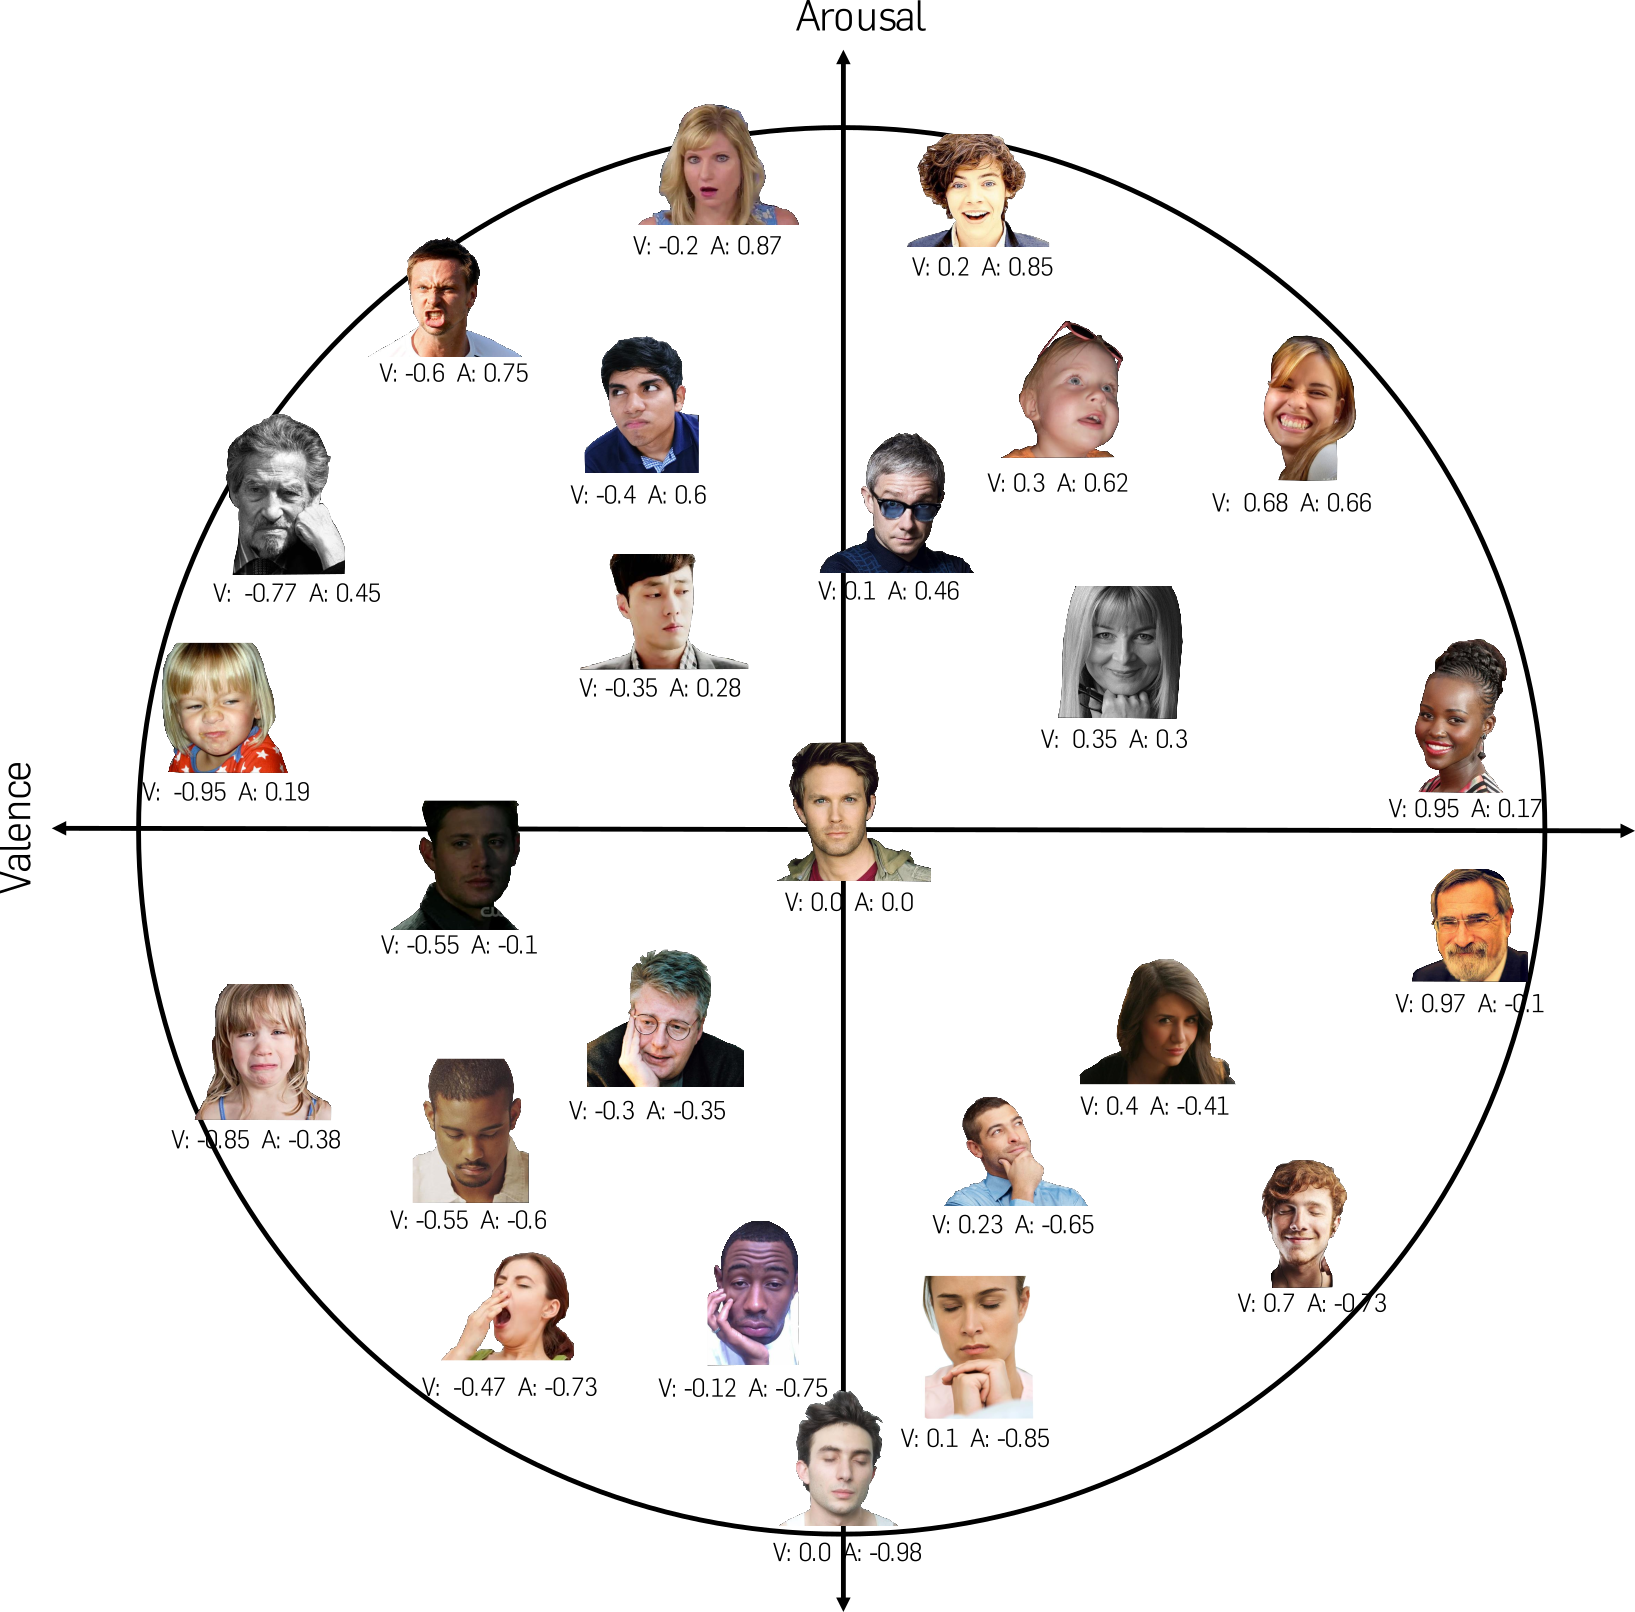
\includegraphics[width=0.8\linewidth]{AffectNet_circumplex}
    \end{center}
\end{frame}

\section{Action Units}

\newcommand{\au}[1]{
    \includegraphics[width=2cm]{au/au-0#1.jpg}
}


{
    \paper{Ekman, {\bf The Facial Action Coding System}, 1977}
\begin{frame}{Facial Action Coding System}

\end{frame}
}

{
    \paper{\source{https://www.cs.cmu.edu/\%7Eface/facs.htm}{Automated Face Analysis group, CMU}}
\begin{frame}{Action Units}
    \begin{center}

    \scriptsize
        \begin{tabular}{@{}p{0.5cm}p{2.5cm}p{3.5cm}p{2.5cm}@{}}
    \toprule
    \textbf{AU} & \textbf{Description} & \textbf{Facial muscle}                                                                   & \textbf{Example image} \\
    \midrule
    \only<1>{
    \textbf{1}  & Inner Brow Raiser    & \textit{Frontalis, pars medialis}                                                        & \au{01}                       \\
    \textbf{2}  & Outer Brow Raiser    & \textit{Frontalis, pars lateralis}                                                       & \au{02}                       \\
    \textbf{4}  & Brow Lowerer         & \textit{Corrugator supercilii, Depressor supercilii}                                     & \au{04}                       \\
    \textbf{5}  & Upper Lid Raiser     & \textit{Levator palpebrae superioris}                                                    & \au{05}                       \\
    \textbf{6}  & Cheek Raiser         & \textit{Orbicularis oculi, pars orbitalis}                                               & \au{06}                       \\
    \bottomrule
    }
    \only<2>{
    \textbf{7}  & Lid Tightener        & \textit{Orbicularis oculi, pars palpebralis}                                             & \au{07}                       \\
    \textbf{9}  & Nose Wrinkler        & \textit{Levator labii superioris alaquae nasi}                                           & \au{09}                       \\
    \textbf{10} & Upper Lip Raiser     & \textit{Levator labii superioris}                                                        & \au{10}                       \\
    \textbf{11} & Nasolabial Deepener  & \textit{Zygomaticus minor}                                                               & \au{11}                       \\
    \textbf{12} & Lip Corner Puller    & \textit{Zygomaticus major}                                                               & \au{12}                       \\
    \bottomrule
    }
    \only<3>{
    \textbf{13} & Cheek Puffer         & \textit{Levator anguli oris (a.k.a. Caninus)}                                            & \au{13}                       \\
    \textbf{14} & Dimpler              & \textit{Buccinator}                                                                      & \au{14}                       \\
    \textbf{15} & Lip Corner Depressor & \textit{Depressor anguli oris (a.k.a. Triangularis)}                                     & \au{15}                       \\
    \textbf{16} & Lower Lip Depressor  & \textit{Depressor labii inferioris}                                                      & \au{16}                       \\
    \bottomrule
    }
    \only<4>{
    \textbf{17} & Chin Raiser          & \textit{Mentalis}                                                                        & \au{17}                       \\
    \textbf{18} & Lip Puckerer         & \textit{Incisivii labii superioris and Incisivii labii inferioris}                       & \au{18}                       \\
    \textbf{20} & Lip stretcher        & \textit{Risorius w/ platysma}                                                            & \au{20}                       \\
    \textbf{22} & Lip Funneler         & \textit{Orbicularis oris}                                                                & \au{22}                       \\
    \textbf{23} & Lip Tightener        & \textit{Orbicularis oris}                                                                & \au{23}                       \\
    \bottomrule
    }
    \only<5>{
    \textbf{24} & Lip Pressor          & \textit{Orbicularis oris}                                                                & \au{24}                       \\
    \textbf{25} & Lips part            & \textit{Depressor labii inferioris or relaxation of Mentalis, or Orbicularis oris}       & \au{25}                       \\
    \textbf{26} & Jaw Drop             & \textit{Masseter, relaxed Temporalis and internal Pterygoid}                             & \au{26}                       \\
    \textbf{27} & Mouth Stretch        & \textit{Pterygoids, Digastric}                                                           & \au{27}                       \\
    \bottomrule
    }
    \only<6>{
    \textbf{28} & Lip Suck             & \textit{Orbicularis oris}                                                                & \au{28}                       \\
    \textbf{41} & Lid droop            & \textit{Relaxation of Levator palpebrae superioris}                                      & \au{41}                       \\
    \textbf{42} & Slit                 & \textit{Orbicularis oculi}                                                               & \au{42}                       \\
    \textbf{43} & Eyes Closed          & \textit{Relaxation of Levator palpebrae superioris; Orbicularis oculi, pars palpebralis} & \au{43}                       \\
    \textbf{44} & Squint               & \textit{Orbicularis oculi, pars palpebralis}                                             & \au{44}                       \\
    \bottomrule
    }
    \only<7>{
    \textbf{45} & Blink                & \textit{Levator palpebrae superioris; Orbicularis oculi, pars palpebralis} &                               \\
    \textbf{46} & Wink                 & \textit{Levator palpebrae superioris; Orbicularis oculi, pars palpebralis} &                               \\
    \textbf{51} & Head turn left       &                                                                                          & \au{51}                       \\
    \textbf{52} & Head turn right      &                                                                                          & \au{52}                       \\
    \bottomrule
    }
    \only<8>{
    \textbf{53} & Head up              &                                                                                          & \au{53}                       \\
    \textbf{54} & Head down            &                                                                                          & \au{54}                       \\
    %\textbf{55} & Head tilt left       &                                                                                          & \au{55}                       \\
    %\textbf{56} & Head tilt right      &                                                                                          & \au{56}                       \\
    \bottomrule
    }
    \only<9>{
    %\textbf{57} & Head forward         &                                                                                          & \au{57}                       \\
    %\textbf{58} & Head back            &                                                                                          & \au{58}                       \\
    \textbf{61} & Eyes turn left       &                                                                                          & \au{61}                       \\
    \textbf{62} & Eyes turn right      &                                                                                          & \au{62}                       \\
    \textbf{63} & Eyes up              &                                                                                          & \au{63}                       \\
    \textbf{64} & Eyes down            &                                                                                          & \au{64}                       \\ 
    \bottomrule
    }
    \end{tabular}
    \end{center}

\end{frame}
}

\begin{frame}{OpenFace Action Units}
    \begin{center}
        \Large \href{https://github.com/TadasBaltrusaitis/OpenFace}{github.com/TadasBaltrusaitis/OpenFace}
        \vspace{2em}

        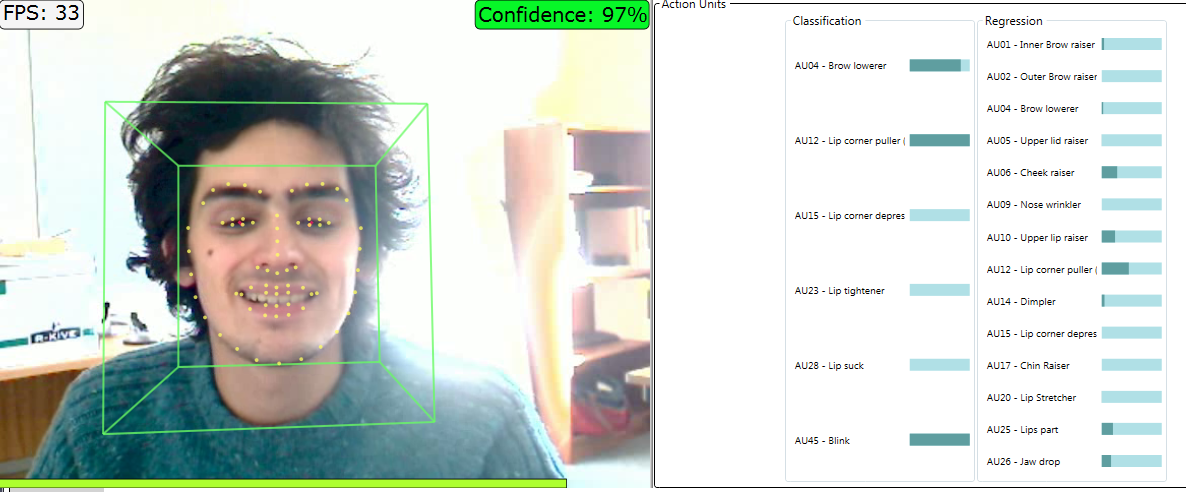
\includegraphics[width=\linewidth]{au_openface}

        \scriptsize
        (not to be confused with this other \href{https://github.com/cmusatyalab/openface}{CMU OpenFace})
    \end{center}
\end{frame}

\begin{frame}{OpenFace 18 Action Units}

    \begin{columns}
        \begin{column}{0.5\linewidth}
    \begin{center}

    \scriptsize
        \begin{tabular}{@{}p{0.3cm}p{2.5cm}p{2cm}@{}}
    \toprule
    \textbf{AU} & \textbf{Description} & \textbf{Example image} \\
    \midrule
    \only<1>{
    \textbf{1}  & Inner Brow Raiser    &  \au{01} \\
    \textbf{2}  & Outer Brow Raiser    &  \au{02} \\
    \textbf{4}  & Brow Lowerer         &  \au{04} \\
    \textbf{5}  & Upper Lid Raiser     &  \au{05} \\
    \textbf{6}  & Cheek Raiser         &  \au{06} \\
    \bottomrule
    }
    \only<2>{
    \textbf{15} & Lip Corner Depressor &  \au{15} \\
    \textbf{17} & Chin Raiser          &  \au{17} \\
    \textbf{20} & Lip stretcher        &  \au{20} \\
    \textbf{23} & Lip Tightener        &  \au{23} \\
    \bottomrule
    }
    \end{tabular}
    \end{center}
            
        \end{column}
        \begin{column}{0.5\linewidth}
    \begin{center}

    \scriptsize
        \begin{tabular}{@{}p{0.3cm}p{2cm}p{2cm}@{}}
    \toprule
    \textbf{AU} & \textbf{Description} & \textbf{Example image} \\
    \midrule
    \only<1>{
    \textbf{7}  & Lid Tightener        &  \au{07} \\
    \textbf{9}  & Nose Wrinkler        &  \au{09} \\
    \textbf{10} & Upper Lip Raiser     &  \au{10} \\
    \textbf{12} & Lip Corner Puller    &  \au{12} \\
    \textbf{14} & Dimpler              &  \au{14} \\
    \bottomrule
    }
    \only<2>{
    \textbf{25} & Lips part            &  \au{25} \\
    \textbf{26} & Jaw Drop             &  \au{26} \\
    \textbf{28} & Lip Suck             &  \au{28} \\
    \textbf{45} & Blink                &          \\
    \bottomrule
    }
    \end{tabular}
    \end{center}
         \end{column}
    \end{columns}

\end{frame}

\begin{frame}{Action Units}



\source{https://en.wikipedia.org/wiki/Facial_Action_Coding_System}{Wikipedia}
\end{frame}

\section{Generating emotional responses}

\imageframe{wall-e}

\begin{frame}{How expressive a robot can be?}

    \begin{columns}
        \begin{column}{0.5\linewidth}
            \begin{center}
                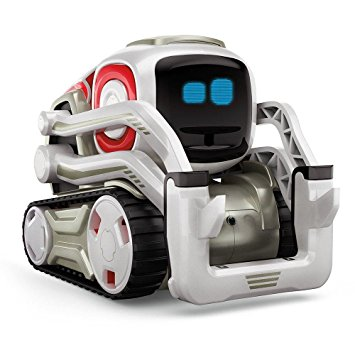
\includegraphics[width=0.8\linewidth]{cozmo}
            \end{center}
        \end{column}
        \begin{column}{0.5\linewidth}
            \href{https://www.anki.com/en-gb/cozmo}{Anki's Cozmo}
        \end{column}
    \end{columns}
\end{frame}

\videoframe[0.56]{figs/cozmo.mp4}

\imageframe[color=black]{cozmo-expression-sheet}


\section{Anthropomorphism}

\imageframe[footnote=Source: Christoph Bartneck,scale=0.9]{bartneck}

\imageframe{anthropo}

\begin{frame}{Dynamics of anthropomorphism}
    \begin{center}
        \includegraphics<1>[width=0.8\linewidth]{dynamics-0}
        \includegraphics<2>[width=0.8\linewidth]{dynamics-1}
        \includegraphics<3>[width=0.8\linewidth]{dynamics-2}
        \includegraphics<4>[width=0.8\linewidth]{dynamics-3}
    \end{center}
\end{frame}

\begin{frame}{Cozmo?}

    \begin{columns}
        \begin{column}{0.4\linewidth}
            \begin{center}
                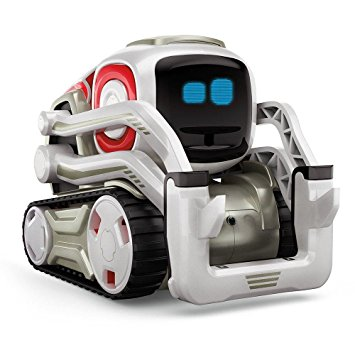
\includegraphics[width=0.8\linewidth]{cozmo}
            \end{center}
        \end{column}
        \begin{column}{0.6\linewidth}
            \begin{center}
                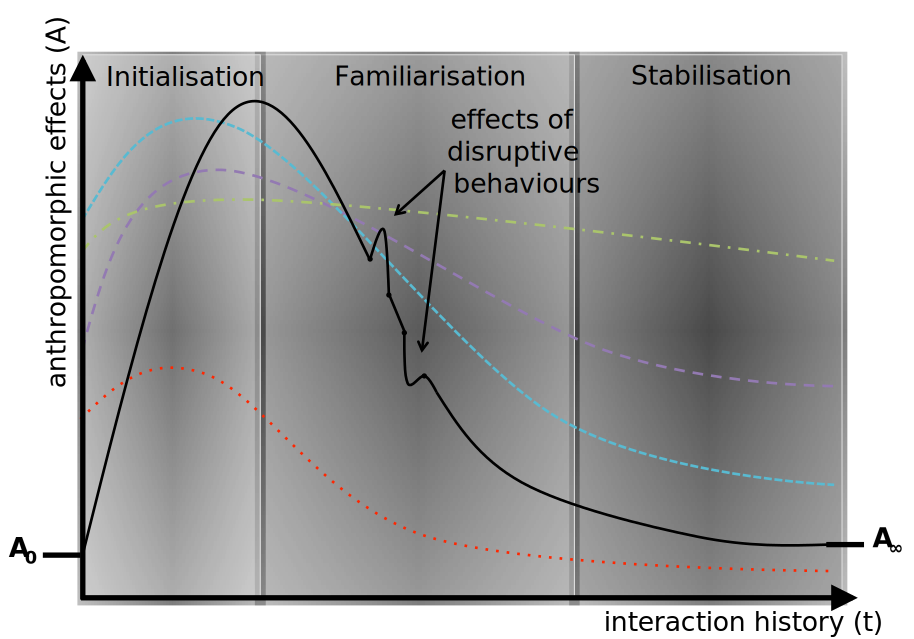
\includegraphics[width=\linewidth]{dynamics-3}
            \end{center}
        \end{column}
    \end{columns}
\end{frame}


\miniframesoff

\begin{frame}{}
    \begin{center}
        \Large
        That's all for today, folks!\\[2em]
        \normalsize
        Questions:\\
        Portland Square B316 or \url{severin.lemaignan@plymouth.ac.uk} \\[1em]

        Slides:\\
        \href{https://github.com/severin-lemaignan/lecture-emotions}{\small
        github.com/severin-lemaignan/lecture-emotions}

    \end{center}
\end{frame}




\end{document}
